% Provenance (never printed): see sources/outline_sources.md (Year 3:
% Glen's flow law; mass balance; ice sheets and ice shelves; sea ice;
% permafrost; the cryosphere's contribution to sea level).
% Brief: sources/book5/BRIEFS.md, ch. 24. Curves from figdata/bachelor-3/
% ice_flow.py (Glen slab, the plastic profile against the ETOPO1 Greenland
% transect, the Arkel ice cap) and sea_ice.py (NSIDC March and September
% extents, Stefan's law). Exercise and problem values in the Book 5 scratch
% calculator calc/ch24.py. The Arkel ice cap and the glaciers of the
% exercises are invented.
\chapter{हिमविज्ञान}\label{ch:b3:glaciology}

ग्रीनलैंड को पश्चिम से पूर्व की ओर, \ang{72.5}N समानांतर के साथ पार करने पर बर्फ़
कुछ दसियों किलोमीटर भीतर से शुरू होती है, तीव्र ढाल से उठती है, फिर उत्तरोत्तर अधिक मंद होती
हुई एक विस्तृत शिखर तक पहुँचती है, जिसकी ऊँचाई \qty{3229}{m} है, और फिर
पूर्वी तट के पर्वतों तक नीचे उतरती है। आलेखित करने पर सतह उस परवलय के लगभग समान है जो
अपनी बगल में पड़ी हो, जिसका शीर्ष किनारे पर हो। यह अध्याय दिखाता है कि वह आकार कहाँ से
आता है: ऐसे पदार्थ से जो अधिक ज़ोर लगने पर उत्तरोत्तर तेज़ी से विसर्पित होता है,
इसलिए वह लगभग ऐसे व्यवहार करता है मानो एक निश्चित प्रतिबल से अधिक सह ही न सकता हो।
इसके बाद यह बर्फ़ का अनुसरण करता है, उस हिम से जो उसे पोषित करता है, उस
समुद्र तक जो उसे ग्रहण करता है।
% ledger: data:b5-etopo-greenland

\begin{recall}
हिमनद, हिमचादरें, हिम-शेल्फ़, हिमशैल, समुद्री हिम, पर्माफ़्रॉस्ट और
हिमयुग स्कूली पुस्तकों में हैं। \omterm{def:b3:deformation-mechanisms:flow-law}{प्रवाह नियम} और \omterm{def:b3:deformation-mechanisms:creep}{अव्यवस्थापन विसर्पण}
अध्याय~\ref{ch:b3:deformation-mechanisms} में हैं; \omterm{def:b3:gravity-geodesy:satgrav}{उपग्रह गुरुत्वमिति} और
हिमचादर द्रव्यमान संतुलन, जिसे वह मापती है, अध्याय~\ref{ch:b3:gravity-geodesy} में;
बर्फ़ का कोर और उसके ऑक्सीजन समस्थानिक अध्याय~\ref{ch:b3:stable-isotopes} में हैं।
समुद्र-तल बजट, हिम--एल्बिडो प्रतिपुष्टि और तापस्थैतिक समुद्र-तल
वृद्धि पुस्तक 4 (स्नातक वर्ष 2) में हैं, उसके मानवजनित
जलवायु परिवर्तन वाले अध्याय में। गुप्त ऊष्मा और ऊष्मा चालन भौतिकी की पुस्तकों में हैं।
\end{recall}

\section{बर्फ़ एक पदार्थ के रूप में}\label{sec:b3:glaciology:material}

हिमनद की बर्फ़ एक चट्टान है, बर्फ़ के परस्पर गुँथे क्रिस्टलों का द्रव्यमान, और
यह अपने गलनांक के निकट विरूपित होती है। प्रतिबल के अधीन यह
अपने क्रिस्टलों में \omterm{def:b3:deformation-mechanisms:dislocation}{अव्यवस्थापन} की गति से विसर्पित होती है, उन चट्टानों की भाँति
अध्याय~\ref{ch:b3:deformation-mechanisms} की, और इसका \omterm{def:b3:deformation-mechanisms:flow-law}{प्रवाह नियम} वही
रूप रखता है: प्रतिबल की एक घात और अर्रेनियस गुणक का गुणनफल।

\begin{theorem}[ग्लेन का प्रवाह नियम]\label{thm:b3:glaciology:glen}
समदैशिक हिमनद-बर्फ़ में विकृति-दर प्रदिश
विचलनात्मक प्रतिबल के समानुपाती होता है,
\[
\dot\varepsilon_{ij} = A(T)\,\tau_e^{\,n-1}\,\tau'_{ij}, \qquad
\tau_e^2 = \tfrac12\,\tau'_{ij}\tau'_{ij},
\]
$n = 3$ के साथ और एक \omterm{def:b3:glaciology:glen}{दर गुणक} $A(T)$, जो तापमान के साथ बढ़ता है।
सरल कर्तन में, जहाँ $\tau_{xz}$ ही एकमात्र अशून्य विचलनात्मक प्रतिबल है,
$\dot\varepsilon_{xz} = A\tau_{xz}^{\,n}$ होता है।
\end{theorem}
\index{ग्लेन का प्रवाह नियम}

\begin{proof}
यह नियम स्वयं अनुभवजन्य है: एक घात नियम जो विसर्पण प्रयोगों और
हिमनदों के विरूपण पर फ़िट किया गया है, और इसका गुणांक तथा घातांक
साथ-साथ निर्धारित किए गए हैं। सरल कर्तन में $\tau'_{xz} = \tau'_{zx} = \tau_{xz}$ और
अन्य घटक शून्य होते हैं, इसलिए $\tau_e^2 = \tfrac12(\tau_{xz}^2 +
\tau_{zx}^2) = \tau_{xz}^2$, और $\dot\varepsilon_{xz} = A\tau_{xz}^{\,n-1}
\tau_{xz}$ है।
\end{proof}
% ledger: pism:rheology

$n = 3$ के साथ बर्फ़ एक प्रबल अरैखिक तरल है: प्रतिबल को दोगुना करने पर वह
आठ गुना तेज़ी से विरूपित होती है। इसकी प्रभावी श्यानता, $1/(2A\tau_e^{\,2})$,
केवल बर्फ़ का गुण नहीं होती, बल्कि प्रतिबल बढ़ने पर घटती है।

\begin{definition}[दर गुणक (बर्फ़)]\label{def:b3:glaciology:glen}
ग्लेन के नियम का \emph{दर गुणक}\index{दर गुणक (बर्फ़)} $A(T)$, जिसे भी
बर्फ़ की मृदुता कहते हैं, $A = A_0\exp(-Q/RT)$ लिखा जाता है, जिसमें
सक्रियण ऊर्जा $Q$ होती है। पैटरसन और बड का व्यापक रूप से प्रयुक्त फ़िट $A_0 =
\qty{3.61e-13}{s^{-1}.Pa^{-3}}$ और $Q = \qty{60}{kJ/mol}$ लेता है, \qty{-10}{\celsius}
से नीचे, और $A_0 = \qty{1.73e3}{s^{-1}.Pa^{-3}}$ और $Q =
\qty{139}{kJ/mol}$ इससे ऊपर, गलनांक के निकट, जहाँ बर्फ़
तापमान के साथ अधिक तेज़ी से मृदु होती है।
\end{definition}
% ledger: pism:rheology, codata:R

\begin{center}
\begin{tabular}{lccc}
\hline
तापमान & \qty{-25}{\celsius} & \qty{-10}{\celsius} & \qty{0}{\celsius}\\
$A$ (\unit{Pa^{-3}.yr^{-1}}) & \num{2.7e-18} & \num{1.4e-17} & \num{1.4e-16}\\
\hline
\end{tabular}
\end{center}

गलनांक पर की बर्फ़ लगभग पचास गुना तेज़ी से बहती है, उसी प्रतिबल के अधीन
\qty{-25}{\celsius} पर की बर्फ़ की तुलना में। हिमनदों में प्रतिबल
एक बार की कोटि का होता है, \qty{e5}{Pa}।
% ledger: pism:rheology

हिमनद दो प्रकार से गति करता है। इसकी बर्फ़ सर्वत्र विसर्पण द्वारा विरूपित होती है; और
जहाँ तल गलनांक पर हो, वहाँ यह फिसल भी सकता है।

\begin{definition}[आधारी सर्पण]\label{def:b3:glaciology:sliding}
\emph{आधारी सर्पण}\index{आधारी सर्पण} हिमनद की अपने तल के ऊपर होने वाली
गति है, जो पानी की पतली फ़िल्म या नम, मृदु अवसाद की परत पर होती है। इसके लिए
गलनांक पर का तल आवश्यक है; तल से जमा हुआ हिमनद केवल
अपनी बर्फ़ के विसर्पण से गति करता है।
\end{definition}
% ledger: nsidc:glacier-flow

\section{हिमनद प्रवाह}\label{sec:b3:glaciology:flow}

\begin{theorem}[समानांतर-पार्श्व स्लैब का प्रवाह]\label{thm:b3:glaciology:slab}
मोटाई $H$ और घनत्व $\rho$ वाली बर्फ़ की एक स्लैब ऐसे तल पर होती है जिसका ढलान
$\alpha$ है, और सरल कर्तन द्वारा उसी पर नीचे बहती है, $u_b$ चाल से फिसलते हुए।
तल से ऊपर ऊँचाई $z$ पर अपरूपण प्रतिबल $\tau = \rho g(H - z)\sin\alpha$ है,
और वेग निम्न है:
\[
u(z) = u_b + \frac{2A}{n + 1}(\rho g\sin\alpha)^n\left[H^{n+1} - (H -
z)^{n+1}\right],
\]
और प्रति इकाई चौड़ाई फ़्लक्स $q = u_bH + \dfrac{2A}{n + 2}(\rho
g\sin\alpha)^nH^{n+2}$ है। आधारी अपरूपण प्रतिबल $\tau_b = \rho gH\sin\alpha$ है।
\end{theorem}

\begin{proof}
ऊँचाई $z$ से ऊपर की हिम का प्रति इकाई क्षेत्रफल भार $\rho g(H - z)$ होता है;
उसका ढलान के अनुदिश घटक, $\rho g(H - z)\sin\alpha$, उसके आधार पर अपरूपण प्रतिबल से संतुलित होता है,
क्योंकि सतह पर कोई प्रतिबल नहीं होता। ग्लेन नियम से,
$\mathrm du/\mathrm dz = 2\dot\varepsilon_{xz} = 2A\tau^n$; आधार से समाकलन करने पर,
जहाँ $u = u_b$ है, $u(z)$ प्राप्त होता है, और $u$ का 0 से $H$ तक समाकलन करने पर
$q$ प्राप्त होता है।
\end{proof}

स्लैब के ऊपरी भाग में वेग बहुत कम बदलता है और आधार के पास तेज़ होता है,
जहाँ प्रतिबल सबसे अधिक होता है: $n = 3$ के साथ अपरूपण
सबसे निचली परतों में केंद्रित रहता है। सतह की गति $H^{n+1} = H^4$ के अनुसार
और ढलान के घन के अनुसार भी बढ़ती है: दोगुनी मोटाई का हिमनद सोलह गुना तेज़ बहता है।

\begin{definition}[उथली-हिम सन्निकटन]\label{def:b3:glaciology:sia}
\emph{उथली-हिम सन्निकटन}\index{उथली-हिम सन्निकटन} ऐसी हिमचादर को, जिसकी मोटाई उसकी चौड़ाई की तुलना में कम हो,
स्थानीय रूप से एक समानांतर-पार्श्व स्लैब मानता है: हर स्थान पर हिम
सरल कर्तन से विरूपित होता है,
\emph{चालक प्रतिबल} $\tau_d = \rho gH|\nabla s|$ के अंतर्गत, जहाँ $s$ सतह की ऊँचाई है,
और फ़्लक्स स्लैब सूत्र का अनुसरण करता है, जिसमें
स्थानीय मोटाई और सतह ढलान का उपयोग होता है।
\end{definition}

\omterm{def:b3:glaciology:sia}{उथली-हिम सन्निकटन} में आधारी प्रतिबल हिम के आकार से तय होता है।
चूँकि विकृति दर प्रतिबल के घन के अनुसार बढ़ती है, प्रतिबल में थोड़ी-सी वृद्धि से
प्रवाह में बड़ी वृद्धि होती है, जिससे हिम पतली हो जाती है और प्रतिबल फिर घट जाता है:
प्रतिबल हिम-द्रव्यमान के आकार चाहे जो हो, एक संकीर्ण परास के भीतर रहता है।
इसे सीमा तक ले जाने पर, ऐसा पदार्थ जो
विराम प्रतिबल $\tau_0$ से नीचे बिल्कुल विरूपित न हो और उससे ऊपर बिना सीमा के विरूपित हो,
तो आकार उसी से निकलता है।

\begin{proposition}[प्लास्टिक हिमचादर प्रोफ़ाइल]\label{prop:b3:glaciology:nye}
विराम प्रतिबल $\tau_0$ वाली पूर्णतः प्लास्टिक हिमचादर, जो एक समतल क्षैतिज आधार पर हो,
अपने सीमांत से अंतर्देशीय दूरी $x$ पर सतह की ऊँचाई इस प्रकार होती है:
\[
h(x) = \sqrt{\frac{2\tau_0x}{\rho g}} .
\]
\end{proposition}
\index{प्लास्टिक हिमचादर प्रोफ़ाइल}

\begin{proof}
हर स्थान पर आधारी प्रतिबल विराम प्रतिबल के बराबर होता है: $\rho gh\,\mathrm
dh/\mathrm dx = \tau_0$, क्योंकि ढलान छोटी है। तब $\mathrm d(h^2)/\mathrm
dx = 2\tau_0/(\rho g)$ होता है, और सीमांत पर $h = 0$ है।
\end{proof}

\begin{omfigure}
\begin{tikzpicture}
\begin{groupplot}[group style={group size=2 by 1, horizontal sep=1.5cm},
  height=0.4\linewidth,
  tick label style={font=\scriptsize}, label style={font=\small}, title style={font=\small}]
\nextgroupplot[width=0.38\linewidth, xlabel={$u/u_s$}, ylabel={आधार से ऊँचाई, $z/H$},
  xmin=0, xmax=1.05, ymin=0, ymax=1, title={स्लैब},
  legend style={font=\scriptsize, at={(0.03,0.97)}, anchor=north west}]
% computed in figdata/bachelor-3/ice_flow.py
\addplot[omThm, thick] table[x=u3, y=zeta] {figdata/out/bachelor-3-ice_flow-slab.dat};
\addlegendentry{$n = 3$}
\addplot[omDef, thick, densely dashed] table[x=u1, y=zeta] {figdata/out/bachelor-3-ice_flow-slab.dat};
\addlegendentry{$n = 1$}
\addplot[omMeth, thick] table[x=u3b, y=zeta] {figdata/out/bachelor-3-ice_flow-slab.dat};
\addlegendentry{$n = 3$, आधारी सर्पण}
\nextgroupplot[width=0.58\linewidth, xlabel={\ang{58}W से \ang{72.5}N के अनुदिश दूरी (\unit{km})},
  ylabel={ऊँचाई (\unit{m})}, xmin=0, xmax=1270, ymin=-500, ymax=3700,
  title={ग्रीनलैंड}, scaled x ticks=false, xticklabel style={/pgf/number format/1000 sep={}},
  scaled y ticks=false, yticklabel style={/pgf/number format/1000 sep={}},
  legend style={font=\scriptsize, at={(0.5,0.03)}, anchor=south}]
\addplot[black, thin] table[x=x, y=h] {figdata/out/bachelor-3-ice_flow-gl.dat};
\addlegendentry{हिम और भूमि सतह}
\addplot[omThm, thick, densely dashed] table[x=x, y=h] {figdata/out/bachelor-3-ice_flow-nye-w.dat};
\addlegendentry{प्लास्टिक प्रोफ़ाइलें}
\addplot[omThm, thick, densely dashed, forget plot] table[x=x, y=h] {figdata/out/bachelor-3-ice_flow-nye-e.dat};
\draw[black!40] (axis cs:0,0) -- (axis cs:1270,0);
\node[font=\scriptsize, omThm, align=center] at (axis cs:330,2900) {$\tau_0 = $\\ \qty{72}{kPa}};
\node[font=\scriptsize, omThm, align=center] at (axis cs:1040,2900) {$\tau_0 = $\\ \qty{108}{kPa}};
\end{groupplot}
\end{tikzpicture}

\par\smallskip{\small बाईं ओर, हिम-स्लैब के पार वेग, सतह की गति से
मापित: ग्लेन नियम ($n = 3$) अपरूपण को आधार के पास केंद्रित करता है, जबकि
रैखिक तरल ($n = 1$) उसे फैलाता है; \omterm{def:b3:glaciology:sliding}{आधारी सर्पण} के साथ पूरी प्रोफ़ाइल खिसक जाती है।
दायीं ओर, \ang{72.5}N के अनुदिश ग्रीनलैंड की सतह (ETOPO1 Ice Surface,
NOAA NCEI), और उसकी दोनों भुजाओं पर फ़िट की गई प्लास्टिक प्रोफ़ाइलें,
\qty{1000}{m} से ऊपर की ऊँचाइयों के लिए और समुद्र-तल पर लिए गए आधार के लिए।
फ़िट के लिए \qty{72}{kPa} और \qty{108}{kPa} के विराम प्रतिबल चाहिए, जो
वास्तविक हिमनदों के बार की कोटि के हैं; वे तीखे सीमांत ढलानों को चूक जाते हैं,
जहाँ आधार और पिघलाव मायने रखते हैं।}\label{fig:b3:glaciology:flow}
\end{omfigure}
% ledger: data:b5-etopo-greenland, pism:rheology

\section{द्रव्यमान संतुलन}\label{sec:b3:glaciology:mass-balance}

हिमनद को हिम से पोषण मिलता है, और वह पिघलने, वाष्पन और, जहाँ वह जल तक पहुँचता है,
वहाँ \omterm{def:b3:glaciology:grounding-line}{हिम-विखंडन} से बर्फ़ खोता है।
% ledger: nsidc:glacier-zones

\begin{definition}[द्रव्यमान संतुलन; संचयन और अपक्षरण क्षेत्र; साम्य-रेखा]\label{def:b3:glaciology:mass-balance}
\emph{हिमनद द्रव्यमान संतुलन}\index{हिमनद द्रव्यमान संतुलन} किसी हिमनद के द्रव्यमान का एक वर्ष में हुआ परिवर्तन है,
जो आम तौर पर जल-तुल्य मीटर में दिया जाता है
और उसके क्षेत्रफल पर औसत होता है। \emph{पृष्ठ द्रव्यमान
संतुलन}\index{पृष्ठ द्रव्यमान संतुलन} उसका वह भाग है जो सतह की प्रक्रियाओं से आता है,
हिमपात घटा पिघलाव, अपवाह और उर्ध्वपातन; शेष हानि
\omterm{def:b3:glaciology:grounding-line}{हिम-विखंडन} से और आधार पर या तैरती बर्फ़ के नीचे पिघलने से होती है।
\emph{संचयन क्षेत्र}\index{संचयन क्षेत्र} सतह का वह भाग है जहाँ
एक वर्ष में पृष्ठ द्रव्यमान संतुलन धनात्मक होता है,
\emph{अपक्षरण क्षेत्र}\index{अपक्षरण क्षेत्र} वह भाग जहाँ वह ऋणात्मक होता है,
तथा \emph{साम्य-रेखा ऊँचाई}\index{साम्य-रेखा ऊँचाई}
(ELA) उन दोनों के बीच की रेखा की ऊँचाई है, जहाँ वह शून्य है।
\end{definition}

\begin{omfigure}
\centering
\begin{tikzpicture}[>=stealth, font=\small, x=1cm, y=1cm]
% bed and surface of a valley glacier, long section
\fill[black!12] (0,0) -- (0,4.6) .. controls (2,3.6) and (6,1.4) .. (11,0) -- cycle;
\fill[omSea!45] (0,4.6) .. controls (2,3.6) and (6,1.4) .. (11,0)
  -- (11,0) .. controls (8,1.0) and (4,3.2) .. (0.6,5.4) -- (0,5.6) -- cycle;
\draw[thick, black!70] (0,4.6) .. controls (2,3.6) and (6,1.4) .. (11,0);
\draw[thick, omDef] (0,5.6) -- (0.6,5.4) .. controls (4,3.2) and (8,1.0) .. (11,0);
% equilibrium line
\draw[omThm, densely dashed, thick] (5.0,2.76) -- (5.0,4.6);
\node[omThm, font=\scriptsize, anchor=south] at (5.0,4.6) {साम्य-रेखा (ELA)};
% balance arrows
\foreach \x/\y in {1.2/5.02, 2.4/4.27, 3.6/3.56} {\draw[->, omDef, thick] (\x,\y+0.55) -- (\x,\y+0.05);}
\foreach \x/\y in {6.4/2.02, 7.6/1.42, 8.8/0.86} {\draw[->, omThm, thick] (\x,\y+0.02) -- (\x,\y+0.52);}
\node[omDef, font=\scriptsize, align=center] at (2.4,6.2) {संचयन क्षेत्र:\\हिम प्राप्त};
\node[omThm, font=\scriptsize, align=center] at (8.6,2.5) {अपक्षरण क्षेत्र:\\बर्फ़ हानि};
% flow lines, computed inside the ice: buried in the accumulation zone, emerging in the ablation zone
\draw[->, black!60] plot[smooth] coordinates {(1.00,5.14) (1.98,4.28) (2.95,3.54) (3.93,2.93) (4.90,2.43) (5.88,2.00) (6.85,1.62) (7.83,1.24) (8.80,0.86)};
\draw[->, black!60] plot[smooth] coordinates {(2.20,4.39) (2.84,3.89) (3.48,3.43) (4.11,3.02) (4.75,2.67) (5.39,2.36) (6.03,2.08) (6.66,1.82) (7.30,1.56)};
\draw[->, black!60] plot[smooth] coordinates {(3.40,3.67) (3.74,3.44) (4.08,3.21) (4.41,3.00) (4.75,2.81) (5.09,2.63) (5.42,2.47) (5.76,2.32) (6.10,2.17)};
\node[font=\scriptsize, anchor=north east] at (10.9,-0.1) {स्नाउट};
\node[font=\scriptsize] at (3.0,1.4) {आधार-शैल};
\end{tikzpicture}

\par\smallskip{\small संतुलन की स्थिति में घाटी-हिमनद का एक योजनाबद्ध
अनुदैर्ध्य काट। साम्य-रेखा के ऊपर हर वर्ष का हिम दब जाता है और
हिमनद के भीतर नीचे ले जाया जाता है; उसके नीचे पृष्ठ हर वर्ष बर्फ़ खोता है और
गहराई से ऊपर उठती बर्फ़ से उसकी पूर्ति होती है। प्रवाह-रेखाएँ (धूसर) \omterm{def:b3:glaciology:mass-balance}{संचयन क्षेत्र} में
नीचे झुकती हैं और \omterm{def:b3:glaciology:mass-balance}{अपक्षरण क्षेत्र} में ऊपर उठती हैं; प्रवाह एक क्षेत्र के अधिशेष को
दूसरे क्षेत्र की कमी तक पहुँचाता है।}\label{fig:b3:glaciology:zones}
\end{omfigure}
% ledger: nsidc:glacier-zones, nsidc:glacier-flow

हिमचादरों और ऊँचे हिमनदों पर हिम एक
ऋतु में बर्फ़ में नहीं बदलता। उसे बाद के हिम से ढक दिया जाता है, वह संपीड़ित होता है और पुनःक्रिस्टलित होता है।

\begin{definition}[फ़िर्न; छिद्र-बंदी]\label{def:b3:glaciology:firn}
\emph{फ़िर्न}\index{फ़िर्न} वह हिम है जो कम से कम एक गलन ऋतु से बच निकला है
और संपीड़ित होकर बर्फ़ में बदल रहा है: यह हिम से सघन होता है, फिर भी वायु के लिए पारगम्य रहता है।
\emph{छिद्र-बंदी}\index{छिद्र-बंदी} संपीड़न का वह बिंदु है, जिस पर
घनत्व लगभग \qtyrange{820}{830}{kg/m^3} होता है, जहाँ कणों के बीच के रंध्र बुलबुलों में बंद हो जाते हैं
और उनकी हवा
वायुमंडल से कट जाती है।
\end{definition}

ध्रुवीय हिमचादरों पर \omterm{def:b3:glaciology:firn}{छिद्र-बंदी}
सतह के नीचे \qtyrange{50}{120}{m} के बीच होती है, जो तापमान, संचयन और अशुद्धियों पर निर्भर करती है;
इसलिए बर्फ़ के कोर के बुलबुलों की हवा उसके आसपास की बर्फ़ से नई होती है,
जैसा अध्याय~\ref{ch:b3:stable-isotopes} में याद किया गया था।
अधिकांश हिमनदों में हिम से बर्फ़ में परिवर्तन में सौ वर्ष से अधिक समय लगता है।
% ledger: nsidc:firn, firn:close-off

हिमनद अपनी जलवायु के बदलाव पर तुरंत प्रतिक्रिया नहीं देता। उसकी मोटाई को पहले
बदलना पड़ता है, तभी उसकी लंबाई उसका अनुसरण कर सकती है।

\begin{proposition}[हिमनद प्रतिक्रिया-काल]\label{prop:b3:glaciology:response}
किसी विशिष्ट मोटाई $H$ वाला हिमनद, जिसके अग्रभाग पर संतुलन $b_t <
0$ (प्रति वर्ष बर्फ़ के मीटरों में) है, जलवायु परिवर्तन के साथ लगभग
इस क्रम के समय में समायोजित होता है:
\[
\tau = \frac{H}{-b_t} .
\]
\end{proposition}

\begin{proof}
हिमनद पर संतुलन में $\delta b$ का परिवर्तन उसके आयतन को तब तक बदलता है
जब तक अग्रभाग पर, जहाँ संतुलन $b_t$ है, खोया या प्राप्त क्षेत्रफल उसकी भरपाई नहीं कर देता,
उसकी भरपाई करता है: प्रति इकाई चौड़ाई $L\,\delta b = -b_t\,\delta L$ होता है,
यह लंबाई $L$ वाले हिमनद के लिए है। आवश्यक आयतन परिवर्तन लगभग $H\,\delta L$ है, और
इसे चलाने वाला असंतुलन आरंभ में प्रति वर्ष $L\,\delta b$ है, इसलिए
परिवर्तन में $H\,\delta L/(L\,\delta b) = H/(-b_t)$ वर्ष लगते हैं।
\end{proof}

\qty{200}{m} मोटा वह हिमनद जो अपने अग्रभाग पर प्रति वर्ष \qty{5}{m} बर्फ़ खोता है,
प्रतिक्रिया देने में लगभग चालीस वर्ष लेता है। इसलिए हिमनद जलवायु से पीछे रहते हैं:
आज के हिमनद, तापमान बढ़ना रुक भी जाए तब भी,
दशकों तक द्रव्यमान खोते रहेंगे।
% ledger: ar6ch9:glaciers

\section{हिमचादर और हिम-शेल्फ़}\label{sec:b3:glaciology:ice-sheets}

ग्रीनलैंड और अंटार्कटिका की हिमचादरें भूमि के हिम का
\qty{99}{\percent} से अधिक रखती हैं। ग्रीनलैंड की चादर \qty{1.7}{\mega
km^2} क्षेत्र में फैली है और अधिकतम रूप से \qty{3}{km} से अधिक मोटी है; अंटार्कटिका की चादर
लगभग \qty{14}{\mega km^2} में फैली है और अधिकतम रूप से लगभग \qty{4.9}{km} मोटी है। अंटार्कटिक हिमचादर के कई भाग
समुद्र-तल से नीचे की भूमि पर टिके हैं।
% ledger: nsidc:ice-sheets, ar6ch9:faq91

\begin{definition}[हिम-धारा]\label{def:b3:glaciology:ice-stream}
एक \emph{हिम-धारा}\index{हिम-धारा} हिमचादर का वह पट्टा है जो अपने दोनों ओर के हिम से
कहीं अधिक तेज़ी से बहता है, मुख्यतः सर्पण द्वारा या
किसी मुलायम गीले आधार के विरूपण द्वारा, और हिमचादर के आंतरिक भाग के बड़े हिस्से को
उसकी सीमा की ओर निकालता है।
\end{definition}

\begin{definition}[भू-स्पर्श रेखा; हिम-विखंडन]\label{def:b3:glaciology:grounding-line}
\emph{भू-स्पर्श रेखा}\index{भू-स्पर्श रेखा} वह रेखा है जहाँ
अपनी शैय्या पर टिका हिम तैरने लगता है: उसके समुद्र की ओर के भाग में हिम हिम-शेल्फ़ या तैरती हिमनद-जीभ होता है।
\emph{हिम-विखंडन}\index{हिम-विखंडन} हिम के खंडों, यानी हिमशैलों, का टूटकर अलग होना है,
हिमनद या हिम-शेल्फ़ के उस अग्रभाग पर होता है,
जो पानी में समाप्त होता है।
\end{definition}

हिम-शेल्फ़ तैरते हैं, इसलिए उनके पिघलने से समुद्र-तल नहीं बढ़ता। परंतु वे
अपने पार्श्वों और समुद्र-तल के उन उभारों पर टिके रहते हैं, जहाँ वे
तल से टकराते हैं, और वहाँ का घर्षण पीछे के हिम के बहाव का विरोध करता है:
वे उसे \emph{अवरोधित} करते हैं। लार्सन~B हिम-शेल्फ़ के 2002 में विघटित होने के बाद,
जिन हिमनदों ने उसे पोषित किया था, उनकी गति आठ गुना तक बढ़ गई।
% ledger: nsidc:ice-shelves

\begin{proposition}[उत्प्लावन]\label{prop:b3:glaciology:flotation}
घनत्व $\rho_i$ और मोटाई $H$ वाला हिम, समुद्र-तल से नीचे गहराई $D$ पर स्थित शैय्या के ऊपर,
घनत्व $\rho_w$ वाले समुद्री पानी में तैरता है यदि $H < (\rho_w/\rho_i)D$।
$\rho_i = \qty{917}{kg/m^3}$ और $\rho_w = \qty{1025}{kg/m^3}$ लेने पर,
\omterm{def:b3:glaciology:grounding-line}{भू-स्पर्श रेखा} वहाँ होती है जहाँ हिम की मोटाई $1.12\,D$ है।
\end{proposition}

\begin{proof}
तैरता हिम अपने भार के बराबर पानी विस्थापित करता है: मोटाई $H$ वाले स्तंभ को
$\rho_iH/\rho_w$ के बराबर धँसाव चाहिए। यदि पानी उस धँसाव से
गहरा है, तो हिम तैरता है।
\end{proof}
% ledger: iapws:ice-density, noaa:seawater-1025

\begin{omfigure}
\centering
\begin{tikzpicture}[>=stealth, font=\small, x=1cm, y=1cm]
% sea and bed
\fill[omSea!50] (4.2,0) rectangle (11,-2.8);
\fill[black!15] (0,-0.9) -- (2.2,-2.0) -- (4.6,-1.6) -- (7.0,-2.3) -- (11,-2.6)
  -- (11,-3.2) -- (0,-3.2) -- cycle;
\draw[thick, black!60] (0,-0.9) -- (2.2,-2.0) -- (4.6,-1.6) -- (7.0,-2.3) -- (11,-2.6);
% grounded ice and ice shelf
\fill[white] (0,-0.9) -- (0,2.4) .. controls (2,2.2) and (3.6,1.4) .. (4.6,0.2)
  -- (9.2,0.12) -- (9.2,-1.0) -- (4.6,-1.6) -- (2.2,-2.0) -- cycle;
\draw[thick, omDef] (0,2.4) .. controls (2,2.2) and (3.6,1.4) .. (4.6,0.2) -- (9.2,0.12)
  -- (9.2,-1.0) -- (4.6,-1.6);
\draw[thick] (0,0) -- (0,0);
\draw[omDef!60, thin] (0,0) -- (4.3,0); \draw[omDef!60, thin] (9.2,0) -- (11,0);
\node[font=\scriptsize, anchor=south west] at (0.05,0.02) {समुद्र-तल};
% icebergs
\fill[white] (10.1,0.1) rectangle (10.6,-0.7); \draw[omDef] (10.1,0.1) rectangle (10.6,-0.7);
% labels
\fill[omThm] (4.6,-1.6) circle (0.07);
\draw[omThm, ->] (4.0,-2.6) node[anchor=north, font=\scriptsize] {भू-स्पर्श रेखा} -- (4.55,-1.68);
\node[font=\scriptsize] at (1.4,1.1) {भूमि पर टिकी हिमचादर};
\node[font=\scriptsize] at (6.9,-0.7) {तैरता हिम-शेल्फ़};
\node[font=\scriptsize, anchor=south] at (9.2,0.2) {हिम-विखंडन अग्र};
\node[font=\scriptsize, anchor=north, align=center] at (10.35,-0.8) {हिमशैल};
\node[font=\scriptsize, align=center] at (2.1,-2.55) {शैय्या अंतर्देशीय\\गहरी होती है};
\draw[->, black!60, thick] (2.2,1.6) -- (3.6,1.0);
\draw[->, black!60, thick] (5.4,-0.2) -- (7.0,-0.2);
\node[font=\scriptsize, align=center, omMeth] at (7.0,1.2) {अवरोधन: शेल्फ़ के पार्श्वों और\\भूमि पर टिके उभारों पर घर्षण};
\draw[->, omMeth, thick] (7.6,0.6) -- (6.6,0.6);
\end{tikzpicture}

\par\smallskip{\small समुद्री हिमचादर का एक योजनाबद्ध खंड, जो
मापनुसार नहीं है। हिम एक ऐसे आधार पर टिकी है जो समुद्र-तल से नीचे है और जो अंतर्देशीय दिशा में गहरा होता जाता है; \omterm{def:b3:glaciology:grounding-line}{भू-स्पर्श रेखा} पर
हिम एक हिम-शेल्फ़ के रूप में तैरने लगती है, जो अपने अग्र भाग पर \omterm{def:b3:glaciology:grounding-line}{हिम-विखंडन} से
और नीचे से गलने से हिम खोती है। जहाँ शेल्फ़ अपने पार्श्वों पर और समुद्र-तल के उभारों पर थमी है, वहाँ उस पर लगने वाला घर्षण
भूमि पर टिकी हिमचादर के प्रवाह का
विरोध करता है।}\label{fig:b3:glaciology:grounding}
\end{omfigure}
% ledger: nsidc:ice-shelves, ar6ch9:misi

जिस आधार की गहराई अंतर्देशीय दिशा में बढ़ती है, उस पर \omterm{def:b3:glaciology:grounding-line}{भू-स्पर्श रेखा} नाज़ुक होती है। जहाँ
पानी गहरा है, वहाँ \omterm{def:b3:glaciology:grounding-line}{भू-स्पर्श रेखा} पर हिम मोटी होती है, क्योंकि उत्प्लावन की शर्त के अनुसार ऐसा होता है; और
स्लैब प्रमेय के अनुसार मोटे स्तंभ का फ़्लक्स उसकी मोटाई के साथ तीव्रता से बढ़ता है। यदि
\omterm{def:b3:glaciology:grounding-line}{भू-स्पर्श रेखा} ऐसी ढलान से पीछे हटती है, तो
वह और मोटी हिम तक पहुँचती है, जो अधिक विसर्जित होती है, तेज़ी से पतली होती है,
और रेखा को और पीछे हटने देती है।

\begin{definition}[समुद्री हिमचादर अस्थिरता]\label{def:b3:glaciology:misi}
\emph{समुद्री हिमचादर अस्थिरता}\index{समुद्री हिमचादर अस्थिरता}
(MISI) वह प्रस्तावित स्व-प्रबलित पश्चगमन है, जो एक हिमचादर की \omterm{def:b3:glaciology:grounding-line}{भू-स्पर्श रेखा} का होता है,
जो अंतर्देशीय दिशा की ओर ढलते आधार पर टिकी हो: हिम-शेल्फ़ के अवरोधन के बिना
ऐसे आधार पर \omterm{def:b3:glaciology:grounding-line}{भू-स्पर्श रेखा} स्वभावतः अस्थिर रहती है
जब तक वह ऊपर की ओर ढलते आधार तक न पहुँच जाए।
\end{definition}

हिम-शेल्फ़ \omterm{def:b3:glaciology:grounding-line}{भू-स्पर्श रेखा} को नीचे की ढलान पर भी अपनी जगह पर रोक सकते हैं।
ऐसे मॉडल जिनमें सभी अंटार्कटिक हिम-शेल्फ़ हटा दिए जाते हैं और उन्हें पुनः बनने नहीं दिया जाता,
500 वर्षों में इस अस्थिरता से \qtyrange{2}{10}{m} \omterm{def:b3:glaciology:sle}{समुद्र-तल तुल्यांक} के बराबर हिम खोते हैं,
जिसमें से \qtyrange{2}{5}{m} पश्चिमी अंटार्कटिका से आता है।
अधिकतर समुद्र-तल से ऊपर के चट्टानी आधार पर टिकी हिमचादरों पर, जैसे
ग्रीनलैंड, मुख्य स्व-प्रबलित प्रक्रिया दूसरी है: जैसे-जैसे सतह
गलती और नीचे बैठती है, वह गर्म वायु में आ जाती है और अधिक गलती है।
% ledger: ar6ch9:misi, ar6ch9:faq91

\begin{definition}[समुद्र-तल तुल्यांक]\label{def:b3:glaciology:sle}
\emph{समुद्र-तल तुल्यांक}\index{समुद्र-तल तुल्यांक} भूमि की हिम के किसी द्रव्यमान का
वह समुद्र-तल-वृद्धि है, जो उसके गलने से वैश्विक माध्य समुद्र-तल में होती,
यदि जल वर्तमान महासागर पर फैल जाए।
\end{definition}

\begin{proposition}[हिम के द्रव्यमान का समुद्र-तल तुल्यांक]\label{prop:b3:glaciology:sle}
समुद्र-तल से ऊपर टिका हिम का द्रव्यमान $M$, क्षेत्रफल $A_o$ वाले महासागर पर
घनत्व $\rho_w$ वाले जल के रूप में फैलाया जाए, तो वह समुद्र-तल को $M/(\rho_wA_o)$ से ऊपर उठाता है:
प्रत्येक \qty{360}{Gt} के लिए लगभग \qty{1}{mm}।
\end{proposition}

\begin{proof}
जल $M/\rho_w$ आयतन घेरता है, जो क्षेत्रफल $A_o$ पर फैला है। हिमचादर द्रव्यमान-संतुलन आकलनों में अपनाए गए
प्रति मिलीमीटर \qty{360}{Gt} के मान से
$A_o\rho_w = \qty{3.6e17}{kg/m}$ है, अर्थात मीठे पानी के घनत्व के जल के लिए
लगभग \qty{3.6e8}{km^2} क्षेत्रफल का महासागर।
\end{proof}
% ledger: data:b5-imbie

समुद्र-तल से नीचे का हिम पहले से समुद्री जल विस्थापित करता है, इसलिए वह कम गिना जाता है:
अंटार्कटिका के \qty{30}{\mega km^3} हिम का \omterm{def:b3:glaciology:sle}{समुद्र-तल तुल्यांक} लगभग
\qty{58}{m} समुद्र-तल के बराबर है, जो उसके द्रव्यमान को
\qty{360}{Gt/mm} से भाग देने पर मिलने वाले मान से कम है।
% ledger: nsidc:ice-sheets

\begin{omfigure}
\centering
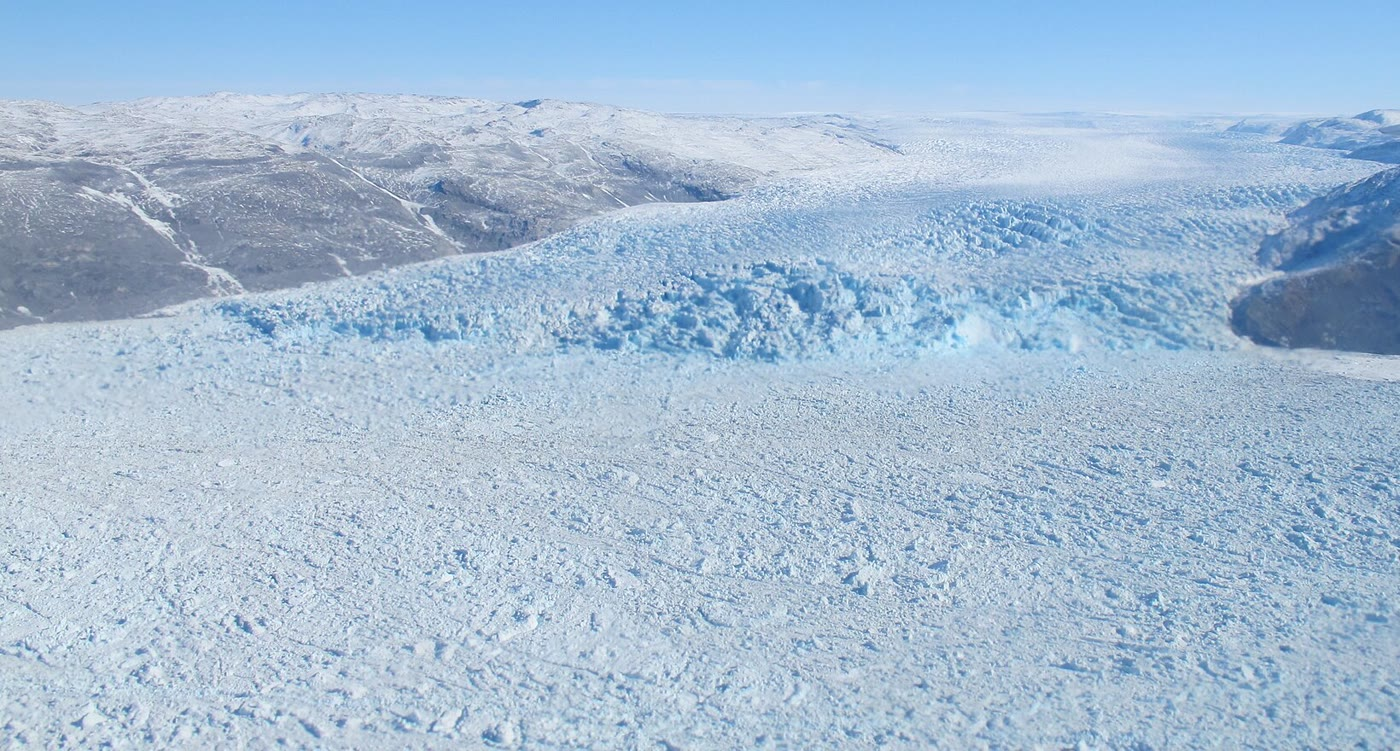
\includegraphics[width=0.82\linewidth]{images/book5/b3-greenland-outlet.jpg}

\par\smallskip{\small ग्रीनलैंड हिमचादर का एक निकास हिमनद,
पर्वतों के बीच से निकलकर अपने \omterm{def:b3:glaciology:grounding-line}{हिम-विखंडन} अग्र पर समुद्र में समाप्त होता है,
चित्र के बीच में नीले हिम की टूटी दीवार दिखती है; सामने का फ़्योर्ड विखंडित हिम और समुद्री हिम से भरा है।
यह फ़ोटो अप्रैल 2014 में NASA के ऑपरेशन आइसब्रिज के एक विमान से
ली गई थी (NASA / Jim Yungel, सार्वजनिक
डोमेन)।}\label{fig:b3:glaciology:outlet}
\end{omfigure}
% ledger: photo:b3-greenland-outlet

\begin{inthefield}[हिम पर एक शिविर]
\begin{minipage}[t]{0.55\linewidth}\vspace{0pt}
हिमचादर पर हिमविज्ञानियों के उपकरण स्लेज से चलते हैं और तंबुओं में
रहते हैं। हिम कितनी तेज़ी से चलती है, यह मापने के लिए वे हिम में एक खंभा जमा देते हैं,
और उस पर एक उपग्रह-नौवहन रिसीवर का एंटीना लगाते हैं।
भूगणित में प्रयुक्त रिसीवर कुछ सेंटीमीटर के भीतर स्थिति तय करते हैं, इसलिए
हफ़्तों या मौसमों में दोहराई गई स्थितियाँ हिम की गति और दिशा बताती हैं,
और खंभे की ऊँचाई, जिसे फिर से सर्वेक्षित किया जाता है,
उसके नीचे की हिम का पतला होना या मोटा होना बताती है।
\end{minipage}\hfill
\begin{minipage}[t]{0.42\linewidth}\vspace{0pt}
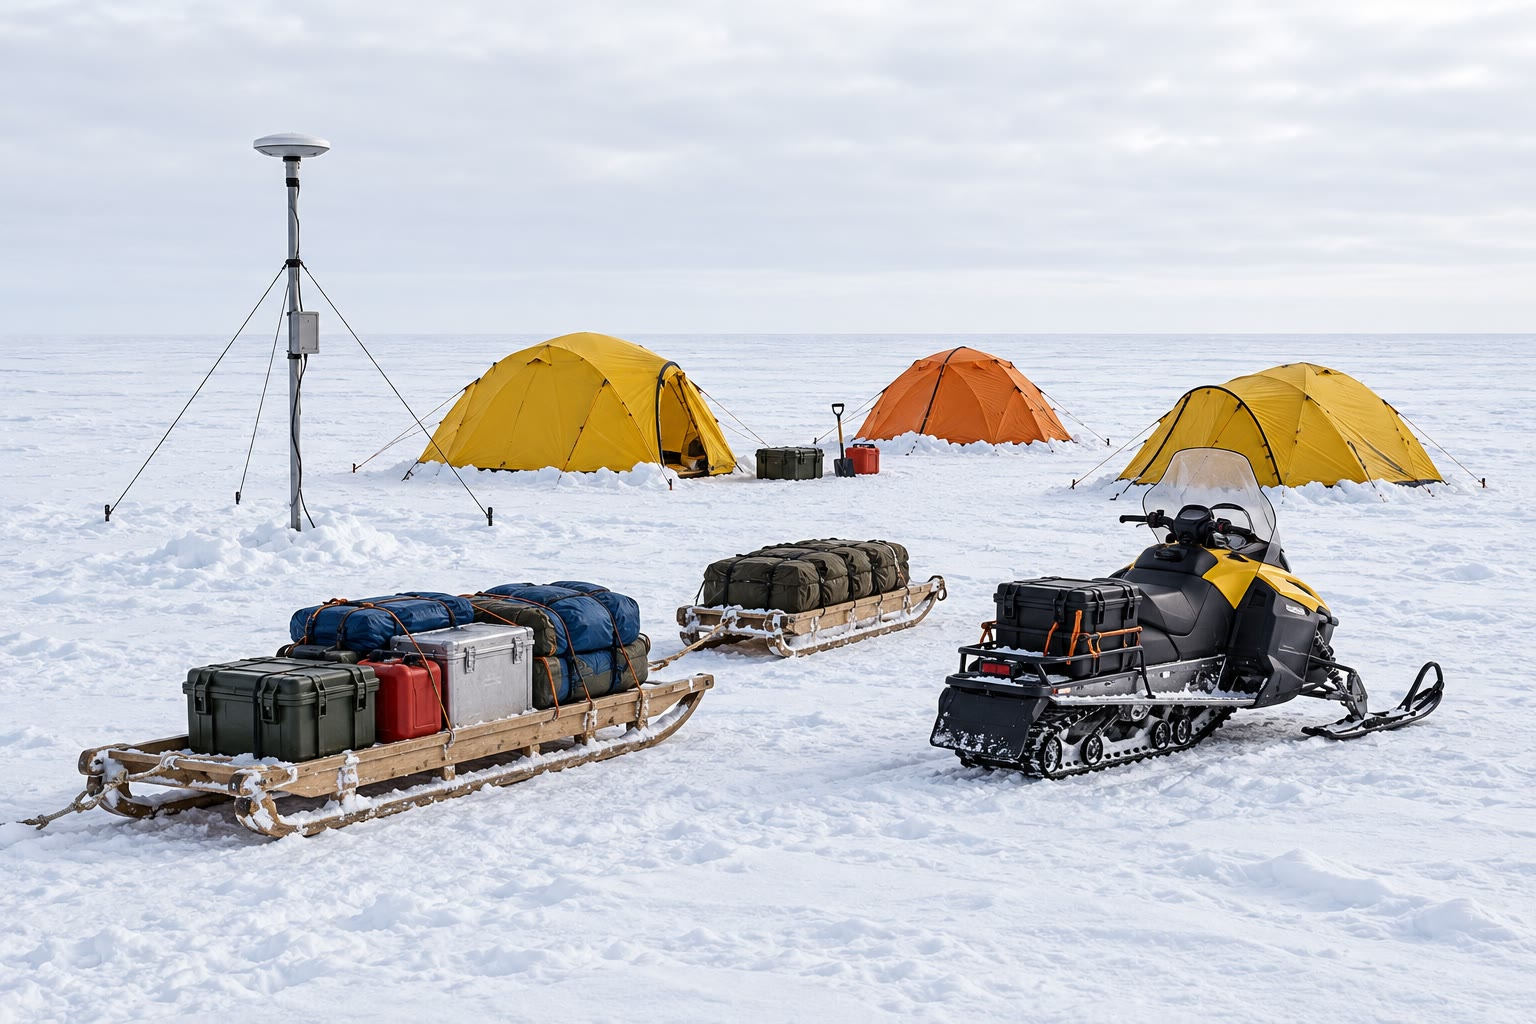
\includegraphics[width=\linewidth]{images/book5/ai/b3-glaciology-camp.jpg}

{\scriptsize हिमचादर पर एक क्षेत्र शिविर: तंबू, स्लेज और एक
स्नोमोबाइल, और एक मस्तूल पर उपग्रह-नौवहन एंटीना, जो टेक-रस्सियों से थमा है
(AI से बनाया गया चित्रण)।}
\end{minipage}
\end{inthefield}
% ledger: gps:high-end

\section{समुद्री हिम और पर्माफ़्रॉस्ट}\label{sec:b3:glaciology:sea-ice}

समुद्री हिम महासागर में बनता है, बढ़ता है और गलता है। आर्कटिक में यह
मार्च में अपने सबसे बड़े क्षेत्रफल तक और सितंबर में अपने सबसे छोटे क्षेत्रफल तक पहुँचता है।
% ledger: nsidc:sea-ice-def

\begin{definition}[समुद्री-हिम विस्तार]\label{def:b3:glaciology:sea-ice}
\emph{समुद्री-हिम विस्तार}\index{समुद्री-हिम विस्तार} उपग्रह मानचित्र की उन कोशिकाओं का
कुल क्षेत्रफल है, जिनमें समुद्री हिम सतह के \qty{15}{\percent} से अधिक भाग को ढकता है।
यह समुद्री-हिम क्षेत्रफल से बड़ा होता है,
जो केवल हिम को गिनता है।
\end{definition}
% ledger: nsidc:sea-ice-def

1979 में उपग्रह द्वारा इसका मानचित्रण आरंभ होने के बाद से आर्कटिक विस्तार सिकुड़ा है, मार्च में
और सितंबर में कहीं अधिक: सितंबर में प्रति दशक \qty{0.74}{\mega km^2} की दर से,
यानी 1981--2010 के माध्य का लगभग \qty{12}{\percent} प्रति दशक, जबकि
मार्च में \qty{0.38}{\mega km^2} प्रति दशक, अर्थात \qty{2.5}{\percent}।
सितंबर का अब तक का सबसे छोटा विस्तार, \qty{3.57}{\mega km^2}, 2012 में था। आर्कटिक समुद्री
हिम \qtyrange{50}{70}{\percent} सूर्य के प्रकाश को परावर्तित करती है, जबकि खुला महासागर लगभग
\qty{6}{\percent} परावर्तित करता है: हिम खोने से सतह अधिक गहरे रंग की हो जाती है,
यह हिम--एल्बिडो प्रतिपुष्टि है, जिसे पुस्तक 4 (स्नातक वर्ष 2) में देखा जा सकता है।
% ledger: data:b5-nsidc-extent, nsidc:sea-ice-reflect

समुद्री हिम अपने निचले तल पर बढ़ती है, जहाँ समुद्र का जल उस पर जमता है, और उस जमाव की गुप्त
ऊष्मा बर्फ़ के भीतर से होकर ऊपर ठंडी हवा तक चालन द्वारा पहुँचनी चाहिए।

\begin{theorem}[स्टीफ़न का नियम]\label{thm:b3:glaciology:stefan}
समुद्री हिम, जिसकी तापीय चालकता $k_i$, घनत्व $\rho_i$ और
संलयन की गुप्त ऊष्मा $L$ है, और जिसकी सतह नीचे के जल के हिमांक से $\Delta T$ नीचे के तापमान पर रखी गई है,
यदि समुद्र से आने वाली ऊष्मा
नगण्य हो, तो इस प्रकार बढ़ती है:
\[
h(t)^2 - h(0)^2 = \frac{2k_i\,\Delta T}{\rho_iL}\,t .
\]
मोटाई $h_s$ और चालकता $k_s$ वाली हिम की परत के नीचे वृद्धि की दर
$\mathrm dh/\mathrm dt = \Delta T/[\rho_iL(h/k_i + h_s/k_s)]$ है।
\end{theorem}

\begin{proof}
पतली बर्फ़ में तापमान रैखिक है, नीचे के हिमांक से
ऊपर सतह के तापमान तक; इसलिए उसमें से ऊष्मा फ़्लक्स
$k_i\Delta T/h$ है, या बर्फ़ और हिम को श्रेणी में लें तो $\Delta T/(h/k_i +
h_s/k_s)$। परत $\mathrm dh$ का जमना प्रति
इकाई क्षेत्रफल $\rho_iL\,\mathrm dh$ ऊष्मा मुक्त करता है, जिसे यह फ़्लक्स दूर ले जाना चाहिए: $\rho_iL\,\mathrm dh/\mathrm dt
= k_i\Delta T/h$। अतः $\mathrm d(h^2)/\mathrm dt = 2k_i\Delta T/(\rho_iL)$।
\end{proof}

$k_i = \qty{2.03}{W.m^{-1}.K^{-1}}$, $L = \qty{3.34e5}{J/kg}$ और
$\rho_i = \qty{917}{kg/m^3}$ के लिए, हिमांक से \qty{20}{K} नीचे की सतह
सौ दिनों में \qty{1.5}{m} और दो सौ दिनों में \qty{2.1}{m} बर्फ़ जमा देती है।
हिम, जिसकी चालकता \qty{0.30}{W.m^{-1}.K^{-1}} है, अच्छी
रोधक है: उसकी \qty{20}{cm} परत वृद्धि को आधे से अधिक घटा देती है। मोटी बर्फ़ धीरे बढ़ती है,
पतली बर्फ़ तेज़; गर्मी में पिघलने के बाद यह नियम
बर्फ़ की मोटाई को समान करने की प्रवृत्ति रखता है।
% ledger: cice:constants, iapws:ice-density

\begin{omfigure}
\begin{tikzpicture}
\begin{groupplot}[group style={group size=2 by 1, horizontal sep=1.5cm},
  width=0.48\linewidth, height=0.4\linewidth,
  tick label style={font=\scriptsize}, label style={font=\small}, title style={font=\small}]
\nextgroupplot[xlabel={वर्ष}, ylabel={विस्तार (\unit{\mega km^2})}, xmin=1977, xmax=2028,
  ymin=0, ymax=18, title={आर्कटिक समुद्री-हिम विस्तार},
  xticklabel style={/pgf/number format/1000 sep={}},
  legend style={font=\scriptsize, at={(0.03,0.66)}, anchor=west}]
% computed in figdata/bachelor-3/sea_ice.py
\addplot[omDef, thick, mark=*, mark size=0.9pt] table[x=year, y=mar] {figdata/out/bachelor-3-sea_ice-extent.dat};
\addlegendentry{मार्च}
\addplot[omThm, thick, mark=*, mark size=0.9pt] table[x=year, y=sep] {figdata/out/bachelor-3-sea_ice-extent.dat};
\addlegendentry{सितंबर}
\addplot[black!60, densely dashed, forget plot] table[x=year, y=mar] {figdata/out/bachelor-3-sea_ice-trend.dat};
\addplot[black!60, densely dashed, forget plot] table[x=year, y=sep] {figdata/out/bachelor-3-sea_ice-trend.dat};
\nextgroupplot[xlabel={जमने के दिन}, ylabel={बर्फ़ की मोटाई (\unit{m})}, xmin=0, xmax=200,
  ymin=0, ymax=2.4, title={वृद्धि, $\Delta T = \qty{20}{K}$},
  legend style={font=\scriptsize, at={(0.97,0.03)}, anchor=south east}]
\addplot[omMeth, thick] table[x=day, y=h0] {figdata/out/bachelor-3-sea_ice-stefan.dat};
\addlegendentry{खुली बर्फ़}
\addplot[omDef, thick, densely dashed] table[x=day, y=hs] {figdata/out/bachelor-3-sea_ice-stefan.dat};
\addlegendentry{\qty{20}{cm} हिम के नीचे}
\end{groupplot}
\end{tikzpicture}

\par\smallskip{\small बाएँ, मार्च और सितंबर में आर्कटिक \omterm{def:b3:glaciology:sea-ice}{समुद्री-हिम का माध्य विस्तार},
1979--2026 (NSIDC सी आइस इंडेक्स, संस्करण~4), न्यूनतम वर्ग
प्रवृत्तियों के साथ (बिंदीदार): \qty{-0.38}{\mega km^2} और \qty{-0.74}{\mega km^2} प्रति
दशक। दाएँ, चालन द्वारा समुद्री हिम की वृद्धि, जिसकी सतह हिमांक से
\qty{20}{K} नीचे है, महासागर की ऊष्मा के बिना: खुली बर्फ़ स्टीफ़न के नियम से,
और वही बर्फ़ \qty{20}{cm} हिम के नीचे।}\label{fig:b3:glaciology:sea-ice}
\end{omfigure}
% ledger: data:b5-nsidc-extent, cice:constants

पर्माफ़्रॉस्ट वह भूमि है जो \qty{0}{\celsius} पर या उससे नीचे
दो या अधिक वर्षों तक रहती है। यह उत्तरी गोलार्ध की उघड़ी भूमि के
लगभग एक-चौथाई भाग के नीचे है।
% ledger: nsidc:permafrost

\begin{definition}[सक्रिय परत]\label{def:b3:glaciology:permafrost}
\emph{सक्रिय परत}\index{सक्रिय परत} पर्माफ़्रॉस्ट के ऊपर की वह भू-परत है
जो हर गर्मी में पिघलती है और हर सर्दी में फिर जम जाती है।
\end{definition}

इसकी मोटाई, समुद्री हिम की वृद्धि की तरह, पिघलने के मौसम में भूमि में
ऊष्मा के चालन से तय होती है, और इसके विरुद्ध भूमि की बर्फ़ की गुप्त ऊष्मा होती है।
पिछले तीन से चार दशकों में सभी पर्माफ़्रॉस्ट क्षेत्रों में पर्माफ़्रॉस्ट के तापमान बढ़े हैं
(उच्च विश्वास); वैश्विक स्तर पर पर्माफ़्रॉस्ट
\qty{0.29}{\celsius} [\numrange{0.17}{0.41}] गर्म हुआ
2007 और 2016 के बीच (मध्यम विश्वास), और \omterm{def:b3:glaciology:permafrost}{सक्रिय परत} की मोटाई में वृद्धि
एक सर्व-आर्कटिक घटना है (मध्यम विश्वास)।
जहाँ इसकी बर्फ़ पिघलती है, वहाँ भूमि धँस सकती है।
% ledger: ar6ch9:permafrost, nsidc:permafrost-thaw

\section{क्रायोस्फ़ीयर और समुद्र-तल}\label{sec:b3:glaciology:sea-level}

पुस्तक 4 (स्नातक वर्ष 2) के समुद्र-तल बजट में गर्म होते महासागर के प्रसार को
बर्फ़ और भूमि से जुड़े जल के साथ जोड़ा जाता है। 2006--2018 में देखे गए
\qty{3.69}{mm/yr} समुद्र-तल उठाव में से हिमनदों ने \qty{0.62}{mm/yr} योगदान दिया,
ग्रीनलैंड ने \qty{0.63}{mm/yr} और अंटार्कटिका ने
\qty{0.37}{mm/yr} योगदान दिया: बर्फ़ का कुल योगदान महासागर के प्रसार,
\qty{1.39}{mm/yr} से अधिक रहा।
% ledger: ar6ch9:table95

\begin{dated}{2021}
ग्रीनलैंड ने 1992--2020 में \qty{4890}{Gt} बर्फ़ खोई [4140 से 5640],
जो \qty{13.5}{mm} समुद्र-तल के बराबर है; उसकी हानि की दर 1990 के दशक में \qty{39}{Gt/yr} से
बढ़कर 2010--2019 में \qty{243}{Gt/yr} हो गई, विसर्जन से और, उत्तरोत्तर,
सतही गलन से (उच्च विश्वास)। अंटार्कटिका ने \qty{2670}{Gt}
[1800 से 3540], \qty{7.4}{mm} खोई, उसकी दर 1990 के दशक में \qty{49}{Gt/yr} से
बढ़कर 2010--2019 में \qty{148}{Gt/yr} हो गई; ये हानियाँ पश्चिमी अंटार्कटिका के
आउटलेट हिमनदों से आईं, मुख्यतः हिम-शेल्फ़ों के नीचे से गलन के कारण (उच्च विश्वास)।
हिमचादरों के बाहर के हिमनदों ने 1993--2019 में \qty{6200}{Gt} खोई,
जो \qty{17.1}{mm} के बराबर है; 2010--2019 में यह रिकॉर्ड के
किसी भी अन्य दशक से अधिक रहा (अति उच्च विश्वास)। ग्रीनलैंड
इस शताब्दी में विचारित सभी परिदृश्यों के अंतर्गत द्रव्यमान खोता रहेगा (लगभग निश्चित), और
अंटार्कटिका भी (संभावित): 2100 तक ग्रीनलैंड संभावित रूप से कम-उत्सर्जन परिदृश्य में समुद्र-तल में
\qtyrange{0.01}{0.10}{m} के बीच जोड़ेगा, और अति-उच्च परिदृश्य में
\qtyrange{0.09}{0.18}{m} के बीच; अंटार्कटिका
\qtyrange{0.03}{0.27}{m} और \qtyrange{0.03}{0.34}{m} के बीच जोड़ेगा।
आर्कटिक महासागर संभावित रूप से व्यावहारिक रूप से समुद्री हिम-मुक्त हो जाएगा;
सितंबर के न्यूनतम पर उसमें \qty{1}{\mega km^2} से कम हिम, पहली बार
विचारित सभी परिदृश्यों के अंतर्गत 2050 से पहले होगा।
\end{dated}
% ledger: ar6ch9:greenland, ar6ch9:antarctica, ar6ch9:glaciers, ar6ch9:ice-sheet-proj, ar6ch9:sea-ice

हिमचादर की हानियाँ वही हैं जो अध्याय~\ref{ch:b3:gravity-geodesy} में
ऊँचाईमापन, गुरुत्वमिति और गिरते हिम तथा बहकर निकलती बर्फ़ के अंतर से मापी गई हैं:
तीन स्वतंत्र विधियाँ
एक ही अनुमान में मिलाई गई हैं।
% ledger: data:b5-imbie

\section{अभ्यास}

\begin{exercise}[$\star$]\label{exo:b3:glaciology:1}
घाटी-हिमनद, जिसकी मोटाई \qty{250}{m} है, \ang{3} के ढाल पर नीचे बहता है। आधारी अपरूपण प्रतिबल
परिकलित कीजिए, और उसकी तुलना वास्तविक हिमनदों के आधारी प्रतिबलों से
कीजिए, जो एक बार की कोटि के हैं।
\end{exercise}

\begin{exercise}[$\star$]\label{exo:b3:glaciology:2}
(क)~ग्रीनलैंड की हिमचादर में लगभग \qty{2.9}{\mega km^3} हिम है, जिसका
घनत्व \qty{917}{kg/m^3} है। इसका द्रव्यमान और \qty{360}{Gt/mm} पर इसका \omterm{def:b3:glaciology:sle}{समुद्र-तल तुल्यांक} परिकलित कीजिए,
और उसकी तुलना प्रायः उद्धृत \qty{7.4}{m} से कीजिए।
(ख)~इसी प्रकार अंटार्कटिका के \qty{30}{\mega km^3} के लिए कीजिए, जिसे लगभग
\qty{58}{m} बताया गया है। ये दोनों परिणाम इतने भिन्न क्यों हैं?
\end{exercise}
% ledger: nsidc:ice-sheets

\begin{exercise}[$\star$]\label{exo:b3:glaciology:3}
एक हिमनद का \omterm{def:b3:glaciology:mass-balance}{संचयन क्षेत्र} \qty{6}{km^2} है, जिसका माध्य संतुलन
\qty{+1.2}{m} जल-तुल्यांक है, और \omterm{def:b3:glaciology:mass-balance}{अपक्षरण क्षेत्र} \qty{4}{km^2} है, जिसका
\qty{-2.1}{m} है। इसका शुद्ध संतुलन घन मीटर जल में, इसका माध्य विशिष्ट संतुलन,
और संचयन-क्षेत्र अनुपात परिकलित कीजिए। क्या यह बढ़ रहा है या
सिकुड़ रहा है?
\end{exercise}

\begin{exercise}[$\star$]\label{exo:b3:glaciology:4}
\omterm{def:b3:glaciology:firn}{छिद्र-बंदी} पर \omterm{def:b3:glaciology:firn}{फ़िर्न} का घनत्व \qtyrange{820}{830}{kg/m^3} के बीच होता है।
इसके आयतन का कितना भाग अभी भी रंध्र-स्थान है (बर्फ़:
\qty{917}{kg/m^3})?
\end{exercise}
% ledger: firn:close-off

\begin{exercise}[$\star\star$]\label{exo:b3:glaciology:5}
समशीतोष्ण हिमनद (बर्फ़ \qty{0}{\celsius} पर, $A =
\qty{1.4e-16}{Pa^{-3}.yr^{-1}}$), जिसकी मोटाई \qty{300}{m} है और जो
\ang{3} के ढाल पर है। केवल आंतरिक विरूपण से इसकी पृष्ठ चाल परिकलित कीजिए।
यदि यह दोगुनी मोटी होती, तो चाल किस गुणक से बदलती? यदि ढाल
आधी होती, तो चाल किस गुणक से बदलती?
\end{exercise}

\begin{exercise}[$\star\star$]\label{exo:b3:glaciology:6}
पैटर्सन--बड स्थिरांकों से \qty{-25}{\celsius} और \qty{-10}{\celsius} पर \omterm{def:b3:glaciology:glen}{दर गुणक}, तथा
\qty{0}{\celsius} और \qty{-25}{\celsius} पर स्थित दो समरूप बर्फ़-पिंडों की चालों का अनुपात
परिकलित कीजिए।
\end{exercise}
% ledger: pism:rheology, codata:R

\begin{exercise}[$\star\star$]\label{exo:b3:glaciology:7}
\qty{1000}{km} दूर, केंद्र से किनारे तक, एक प्लास्टिक हिमचादर की अधिकतम मोटाई
$\tau_0 = \qty{100}{kPa}$ के साथ परिकलित कीजिए, और उसकी तुलना अंटार्कटिका के
हिम की अधिकतम मोटाई से कीजिए, जो लगभग \qty{4.9}{km} है।
\end{exercise}
% ledger: nsidc:ice-sheets

\begin{exercise}[$\star\star$]\label{exo:b3:glaciology:8}
एक हिमनद, जिसकी मोटाई \qty{200}{m} है, अपने अग्र-सिरे पर प्रति वर्ष
\qty{5}{m} हिम खोता है। इसके अनुक्रिया काल का अनुमान लगाइए।
यदि जलवायु अचानक गरम हो गई और फिर स्थिर रही, तो उसकी लंबाई कितने समय तक बदलती रहेगी?
\end{exercise}

\begin{exercise}[$\star\star$]\label{exo:b3:glaciology:9}
(क)~स्टेफ़न के नियम से $\Delta T = \qty{20}{K}$ लेते हुए, 100 दिन बाद नंगे समुद्री हिम की
मोटाई, तथा \qty{3}{m} तक पहुँचने में लगने वाला समय परिकलित कीजिए।
(ख)~इससे \qty{3}{m} से मोटे हिम के बारे में क्या संकेत मिलता है?
\end{exercise}
% ledger: cice:constants

\begin{exercise}[$\star\star\star$]\label{exo:b3:glaciology:10}
(क)~जहाँ तल समुद्र-तल से \qty{800}{m} नीचे है, वहाँ \omterm{def:b3:glaciology:grounding-line}{भू-स्पर्श रेखा} पर हिम कितना
मोटा है? (ख)~स्लैब फ़्लक्स $q \propto H^{n+2}$ का प्रयोग करते हुए, किसी दिए गए
पृष्ठ ढाल के लिए, यदि \omterm{def:b3:glaciology:grounding-line}{भू-स्पर्श रेखा} उस स्थान तक पीछे हटे जहाँ तल \qty{900}{m} गहरा है,
तो भू-स्पर्शी हिम का फ़्लक्स किस गुणक से बढ़ेगा? (ग)~समझाइए कि
अंतर्देशीय तल का गहराना पीछे हटने को स्वयं-प्रबल क्यों बनाता है,
और हिम-शेल्फ़ क्या बदलता है।
\end{exercise}
% ledger: iapws:ice-density, noaa:seawater-1025

\begin{exercise}[$\star\star\star$]\label{exo:b3:glaciology:11}
सिद्ध कीजिए कि त्रिज्या $R$ वाली एक वृत्ताकार प्लास्टिक हिम-टोपी का आयतन $V =
\frac{8\pi}{15}\sqrt{2\tau_0/(\rho g)}\,R^{5/2}$ है। यदि इसकी त्रिज्या दोगुनी हो जाए,
तो इसका \omterm{def:b3:glaciology:sle}{समुद्र-तल तुल्यांक} किस गुणक से बढ़ेगा?
\end{exercise}

\begin{exercise}[$\star\star\star$]\label{exo:b3:glaciology:12}
मार्च 1979 में आर्कटिक का माध्य विस्तार \qty{16.34}{\mega km^2} था, और
मार्च 2026 में \qty{14.13}{\mega km^2}; सितंबर में \num{7.05} और
\qty{4.81}{\mega km^2} था। (क)~प्रत्येक माह में सापेक्ष परिवर्तन परिकलित कीजिए।
(ख)~दो भौतिक कारण बताइए कि सितंबर का विस्तार
मार्च के विस्तार की तुलना में इतनी अधिक तेज़ी से क्यों घटा है।
\end{exercise}
% ledger: data:b5-nsidc-extent

\section{समस्या: आर्केल हिम-टोपी}

\begin{problem}[{सप्ताहांत समस्या --- आकार, प्रवाह, संतुलन और
काल्पनिक हिम-टोपी का समुद्र-तल तुल्यांक}]
\label{pb:b3:glaciology:1}
काल्पनिक आर्केल हिम-टोपी एक समतल पठार पर स्थित है। यह लगभग वृत्ताकार है,
त्रिज्या \qty{20}{km} है, और इसकी बर्फ़ लगभग \qty{-10}{\celsius} पर है। मान लीजिए
$\rho = \qty{917}{kg/m^3}$ और $g = \qty{9.81}{m/s^2}$।

\medskip\noindent\textbf{भाग I --- क्या टोपी प्लास्टिक है?}
\begin{enumerate}
\item सिद्ध कीजिए कि मोटाई $H$ के हिम के नीचे, जिसका पृष्ठ ढाल
  $\alpha$ छोटा हो, तो आधारी अपरूपण प्रतिबल लगभग $\rho gH\alpha$ होता है।
\item केंद्र से 5, 10 और \qty{15}{km} दूरी पर रडार-मापन और सर्वेक्षण
  से मोटाइयाँ 580, 470 और \qty{335}{m} तथा पृष्ठ ढाल
  \num{0.0190}, \num{0.0240} और \num{0.0330} प्राप्त होते हैं। तीनों बिंदुओं पर आधारी अपरूपण
  प्रतिबल परिकलित कीजिए।
\item क्या टोपी प्लास्टिक के निकट है? आप कौन-सा विराम प्रतिबल अपनाते हैं?
\item $\tau_0 = \qty{100}{kPa}$ लेकर $2\tau_0/(\rho g)$ परिकलित कीजिए।
\item प्लास्टिक परिच्छेद से तीनों बिंदुओं पर मोटाई का पूर्वानुमान लगाइए
  और उसकी तुलना रडार-मापनों से कीजिए।
\end{enumerate}

\medskip\noindent\textbf{भाग II --- आकार और आयतन।}
\begin{enumerate}[resume]
\item केंद्र पर मोटाई परिकलित कीजिए।
\item सिद्ध कीजिए कि आयतन $V = \frac{8\pi}{15}\sqrt{2\tau_0/(\rho
  g)}\,R^{5/2}$ है।
\item आयतन घन किलोमीटर में परिकलित कीजिए।
\item क्षेत्रफल और माध्य मोटाई परिकलित कीजिए।
\item उसी पठार पर दोगुनी चौड़ाई की एक हिम-टोपी के लिए, उसका आयतन किस गुणक से
  बड़ा होगा?
\end{enumerate}

\medskip\noindent\textbf{भाग III --- प्रवाह और संतुलन।}
\begin{enumerate}[resume]
\item \qty{-10}{\celsius} पर \omterm{def:b3:glaciology:glen}{दर गुणक}
  \unit{Pa^{-3}.yr^{-1}} में परिकलित कीजिए।
\item केंद्र से \qty{10}{km} दूरी पर, हिम को स्लैब मानकर,
  आंतरिक विरूपण द्वारा सतही चाल परिकलित कीजिए।
\item वहाँ प्रति एकक चौड़ाई का हिम-फ़्लक्स, और
  स्तंभ का माध्य वेग परिकलित कीजिए।
\item स्थायी अवस्था में, त्रिज्या
  \qty{10}{km} के वृत्त से निर्गत फ़्लक्स उसके भीतर प्राप्त संतुलन के बराबर है। इसके लिए
  प्रति वर्ष हिम के मीटर में कितने माध्य संतुलन की आवश्यकता होगी?
\item साम्य-रेखा पठार से \qty{450}{m} ऊँचाई पर स्थित है। यह टोपी पर कहाँ है,
  और संचयन-क्षेत्र अनुपात क्या है?
\item यदि हिम \qty{0}{\celsius} तक गर्म हो जाए, तो चालें किस गुणक से
  बढ़ेंगी? टोपी के आकार का क्या होगा?
\end{enumerate}

\medskip\noindent\textbf{भाग IV --- समुद्र-तल।}
\begin{enumerate}[resume]
\item टोपी का द्रव्यमान गीगाटन में परिकलित कीजिए।
\item इसका \omterm{def:b3:glaciology:sle}{समुद्र-तल तुल्यांक} मिलीमीटर में परिकलित कीजिए।
\item यदि पूरी टोपी प्रति वर्ष \qty{0.5}{m} हिम से पतली हो जाए, बिना बहे,
  तो वह कितने समय तक टिकेगी?
\item वास्तविक टोपी पतली होना शुरू होने पर उससे पहले
  क्यों लुप्त हो जाएगी?
\item 2010--2019 में ग्रीनलैंड जिस दर से हिम खो रहा था, उसी दर पर
  अर्केल टोपी के बराबर द्रव्यमान खोने में कितना समय लगेगा?
\item अर्केल हिम-टोपी का \omterm{def:b3:glaciology:sle}{समुद्र-तल तुल्यांक} मिलीमीटर में,
  एक दशमलव स्थान तक दीजिए।
\end{enumerate}
\end{problem}
% ledger: pism:rheology, data:b5-imbie, ar6ch9:greenland, ar6ch9:faq91
